\documentclass[xcolor=table]{beamer}

\usepackage{subfig}

\usepackage{url}


\usepackage[utf8]{inputenc}
\usepackage[spanish, es-tabla, activeacute]{babel}

\usepackage{amsmath}

\usetheme[ pageofpages=of,% String used between the current page and the
                         % total page count.
          bullet=circle,% Use circles instead of squares for bullets.
          titleline=true,% Show a line below the frame title.
          alternativetitlepage=false,% Use the fancy title page.
          titlepagelogo=unl,% Logo for the first page.
          watermark=imagenes/agua-unl,% Watermark used in every page.
          watermarkheight=90px,% Height of the watermark.
          watermarkheightmult=4,% The watermark image is 4 times bigger
                                % than watermarkheight.
          ]{Torino}


% Personalizacion de colores en bullets
%\definecolor{darkred}{RGB}{161,28,47}
\definecolor{darkorange}{RGB}{230,65,0}
\definecolor{darkbrown}{RGB}{150,75,0}
%\definecolor{darkblue}{RGB}{0,83,197}
\definecolor{darkgreen}{RGB}{0,120,0}

\setbeamerfont{section number projected}{%
	family=\rmfamily,series=\bfseries,size=\normalsize}
%\setbeamercolor{section number projected}{bg=darkorange,fg=white}
%\setbeamercolor{item projected}{bg=darkorange}

\setbeamercolor{title}{fg=white, bg=darkgreen}    % define infoline 1st box color

% Configuro theme y color
\usetheme[secheader]{Boadilla}
%\usetheme{Copenhagen}

\usecolortheme[named=darkgreen]{structure}

\author{Francisco Yackel \and
		\\ \hfil \\
		Director: Dr. Leandro D. Vignolo \and 
		\\
		Co-Director: Ing. Leandro Ferrado}

\subtitle{Desarrollo de una aplicación Android, asistida por visión artificial, para administrar imágenes almacenadas en un dispositivo móvil}
\title{Proyecto Final de Carrera}

\institute{Facultad de Ingeniería y Ciencias Hídricas, \\ Universidad Nacional del Litoral} %\\

\titlegraphic{
\includegraphics[height=1.2cm]{imagenes/logo-fich}}

%\date{5 de Septiembre del 2016}



%-----------------------------------------
% Definición de comandos útiles
\setbeamertemplate{navigation symbols}{}


\makeatletter
\setbeamertemplate{footline}
{
	\leavevmode%
	\hbox{%
		\begin{beamercolorbox}[wd=.3\paperwidth,ht=2.25ex,dp=1ex,center]{date in head/foot}%
			\usebeamerfont{date in head/foot}
			FICH - UNL
			
		\end{beamercolorbox}%
		\begin{beamercolorbox}[wd=.4\paperwidth,ht=2.25ex,dp=1ex,center]{author in head/foot}%
			\usebeamerfont{author in head/foot}
			PFCII 2019
		\end{beamercolorbox}}%
		\begin{beamercolorbox}[wd=.3\paperwidth,ht=2.25ex,dp=1ex,right]{date in head/foot}%
			\usebeamerfont{date in head/foot}\insertshortdate{}\hspace*{2em}
			\insertframenumber{} / \inserttotalframenumber\hspace*{2ex}
		\end{beamercolorbox}%
		\vskip0pt%
	}
	\makeatother
	
	\date[10/03/19]{\tiny 10 de Marzo del 2019}
	
	
	%\AtBeginSection[]
	%{ 
	%	\begin{frame}
	%		\frametitle{Agenda}
	%		\tableofcontents[currentsection]
	%	\end{frame}
	%}

\usepackage{xcolor}

% [Agregado] Para ajustar tablas al tamaño del texto (http://tex.stackexchange.com/questions/163246/resize-a-tabular-object-to-textwidth)
\usepackage{adjustbox}

% [Agregado] Para hacer pie plots con tikzpicture: https://code.google.com/archive/p/pgf-pie/
\usepackage{pgf-pie}


% [Agregado] Package de maths para alinear ecuaciones
\usepackage{amsmath}


% [Agregado] Para hacer histogramas en Figuras
\usepackage{xcolor}
\usepackage{pgfplots}
\usepackage{tikz}

% [Agregado] Para resolver el problema de tener muchos paquetes cargados: http://tex.stackexchange.com/questions/38607/no-room-for-a-new-dimen
\usepackage{etex}

% [Agregado] Para hacer la tabla p/ matriz de confusion
\usepackage{array}
\usepackage{multirow}



% Custom colors
\usepackage{color}
\definecolor{deepblue}{rgb}{0,0,0.5}
\definecolor{deepred}{rgb}{0.6,0,0}
\definecolor{deepgreen}{rgb}{0,0.5,0}
\definecolor{bblue}{HTML}{4F81BD}
\definecolor{rred}{HTML}{C0504D}
\definecolor{ggreen}{HTML}{9BBB59}
\definecolor{ppurple}{HTML}{9F4C7C}

\begin{document}
% DO NOT COMPILE THIS FILE DIRECTLY!
% This is included by the other .tex files.

\begin{frame}[t,plain]
\titlepage
\end{frame}

\watermarkon

\begin{frame}
	\frametitle{Agenda}
	
	\tableofcontents[]
\end{frame}
\watermarkoff


%#######################################################

\section{Conceptos básicos}
%---------------------------------------

% RESUMEN:

%El aprendizaje profundo (conocido en inglés como \textit{deep learning}) es una rama de la inteligencia artificial que, debido al éxito de su utilización en problemas de gran complejidad, se ha vuelto popular y ampliamente desarrollado tanto a nivel empresarial como en el campo de la investigación. Se basa en el diseño de redes neuronales capaces de aprender a extraer características sobre los datos presentados, para así lograr con mayor precisión tareas de clasificación o regresión. La profundidad mencionada en su denominación se debe a que las arquitecturas implementadas suelen componerse de numerosos niveles, con el fin de obtener representaciones de los datos que sean adecuadas para el objetivo planteado sobre la red.

%El problema que presenta implementar esta técnica es el elevado costo computacional comprendido en la construcción de la arquitectura profunda, que ocurre especialmente cuando se trata con cantidades masivas de datos. Además, el hecho de manejar una gran cantidad de hiper-parámetros y sus posibles combinaciones incrementa la dificultad de encontrar de forma rápida una red neuronal adecuada para el problema tratado.

%En este proyecto se plantea como objetivo general el desarrollo de un framework que ofrezca la posibilidad de entrenar redes neuronales mediante los algoritmos y funcionalidades más populares del aprendizaje profundo, y reducir el esfuerzo de diseño y modelado utilizando herramientas de cómputo en paralelo. Esto último implica poder distribuir el trabajo computacional tanto a nivel local sobre los núcleos de un procesador, como también sobre los nodos que componen un clúster. Además se define como un objetivo específico evaluar la potencialidad del software desarrollado mediante su aplicación en tareas de alta complejidad, particularmente en problemas de clasificación sobre datos de electroencefalografía.


%--------------------------------------- 
\subsection{Introducción}
%---------------------------------------

\watermarkon
\begin{frame}
	\frametitle{Agenda}
	
	\tableofcontents[currentsection,currentsubsection]
\end{frame}
\watermarkoff


%---------------------------------------
\begin{frame}[t,fragile]
	\frametitle {Motivación }
	
%	\begin{itemize}
%		\item El constante avance de las tecnologías de comunicación permite que la transmisión de información multimedia sea un aspecto común y diario para las personas que utilizan dispositivos móviles.   
%	\end{itemize}
%	\vspace{10mm}
%	\begin{tabular}{cl}  
%	\begin{tabular}{l}
%		\parbox{0.5\linewidth}{
%			\begin{itemize}
%				\item La transmisión de información multimedia es un aspecto común y diario.
%			\end{itemize}
%			\begin{figure}[t]
%				\begin{center}
%					\includegraphics[width=0.5\textwidth]%
%					{imagenes/redes-sociales}
%				\end{center}
%			\end{figure}
%			\begin{itemize}
%				\item Las tareas llevadas a cabo para organizar las imágenes consumen mucho tiempo y esfuerzo.
%			\end{itemize}
%			\begin{figure}[t]
%				\begin{center}
%					\includegraphics[width=0.5\textwidth]%
%					{imagenes/tareas-administracion}
%				\end{center}
%			\end{figure}
%		}
%	\end{tabular} 
%	&
%	\begin{tabular}{c}
%		
\includegraphics[width=5cm]{imagenes/imachineapp-logo}
%	\end{tabular}
%	\\
%\end{tabular}
\begin{itemize}
	\item La transmisión de información multimedia es un aspecto común y diario.
\end{itemize}
\begin{figure}[t]
	\begin{center}
		\includegraphics[width=0.5\textwidth]%
		{imagenes/redes-sociales}
	\end{center}
\end{figure}
\begin{itemize}
	\item Las tareas llevadas a cabo para organizar las imágenes consumen mucho tiempo y esfuerzo.
\end{itemize}
\begin{figure}[t]
	\begin{center}
		\includegraphics[width=0.5\textwidth]%
		{imagenes/tareas-administracion}
	\end{center}
\end{figure}
	
\end{frame}	

%---------------------------------------
%\begin{frame}[t,fragile]
%	\frametitle {Motivación}	
%	
%	
%	\begin{itemize}
%		\item Cuando se quieren administrar los archivos de un dispositivo móvil, para liberar espacio de almacenamiento o bien al realizar una copia de seguridad, las tareas llevadas a cabo para organizar las imágenes consumen mucho tiempo y esfuerzo.
%	\end{itemize}
%	\vspace{10mm}
%	\begin{figure}[t]
%		\begin{center}
%			\includegraphics[width=1\textwidth]%
%			{imagenes/tareas-administracion}
%		\end{center}
%	\end{figure}
%
%	
%\end{frame}
%---------------------------------------
%\begin{frame}[t,fragile]
%	\frametitle {Motivación}
%	
%	\begin{itemize}
%		\item Se consideró posible obtener una aplicación que cuente con propiedades adecuadas para lograr un agrupamiento automático de los datos tratados. En este caso: \textbf{imágenes}.
%	\end{itemize}
%%	\vspace{10mm}
%	\begin{figure}[t]
%		\begin{center}
%			\includegraphics[width=0.4\textwidth]%
%			{imagenes/imachineapp-logo}
%		\end{center}
%	\end{figure}
%\end{frame}

%---------------------------------------
\begin{frame}[t,fragile]
\frametitle {Objetivos}


\begin{itemize}
	\item Desarrollar una aplicación móvil que, a partir de imágenes almacenadas en el dispositivo, sugiera una estructura de directorios para organizar el conjunto.
	
	\item Proveer al sistema funcionalidades que le permitan al usuario la interacción con el resultado, para desempeñar distintas tareas de administración.
\end{itemize}

\begin{figure}[t]
	\begin{center}
		\includegraphics[width=0.3\textwidth]%
		{imagenes/imachineapp-logo}
	\end{center}
\end{figure}
\end{frame}

\begin{frame}[t,fragile]
\frametitle {Alcance}
\begin{itemize}
	\item Desarrollar de manera \textbf{nativa} la aplicación para el sistema operativo Android.
	\vspace{2mm}
	\item Implementar el algoritmo de procesamiento y agrupación de imágenes \textbf{on premise}.
	\vspace{2mm}
	\item Asistir al usuario, brindando \textbf{herramientas de administración} para que pueda interactuar con el resultado.
	\vspace{2mm}
	\item Procesar un total de \textbf{400 imágenes} por ejecución.
\end{itemize}


\end{frame}

%--------------------------------------- 
\subsection{Fundamentos teóricos}
%---------------------------------------

\watermarkon
\begin{frame}
\frametitle{Agenda}

\tableofcontents[currentsection,currentsubsection]
\end{frame}
\watermarkoff

%---------------------------------------
\begin{frame}[t,fragile]
	\frametitle {Machine learning}
	
	\begin{block}{}
		\textit{Abarca algoritmos y técnicas para construir sistemas que son capaces de aprender a partir de datos y a realizar diversos tipos de tareas, sin requerir que se les indique \textbf{cómo} hacerlas.}
	\end{block}
	\vspace{10mm}
	\begin{figure}[t]
		\begin{center}
			\includegraphics[width=0.6\textwidth]%
			{imagenes/machinelearningnewparadigm}
		\end{center}
	\end{figure}
	
%	\begin{tabular}{cl}  
%		\begin{tabular}{l}
%			\parbox{0.5\linewidth}{
%				\begin{itemize}
%					\item Los sistemas por lo general siguen dos tipos de aprendizaje: \color{red}{supervisado} \color{black} y 
%					\color{blue}no supervisado\color{black}.
%					
%				\item Las tareas a realizar suelen clasificarse en estas categorías: 
%				
%				\begin{itemize}
%					\color{red} % SUPERVISADO
%					\item Clasificación
%					\item Regresión
%					
%					\color{blue} % NO SUPERVISADO
%					\item Clustering
%				\end{itemize}
%					
%%				\item Casos de aplicación: DEFINIR COMO EJEMPLOS
%%					\begin{itemize}
%%						\item Visión computacional
%%						\item Motores de búsqueda
%%						\item Reconocimiento de voz
%%					\end{itemize}
%				\end{itemize}
%			}
%		\end{tabular} 
%		&
%		\begin{tabular}{c}
%			
\includegraphics[width=5cm]{imagenes/machinelearningnewparadigm}
%		\end{tabular}
%		\\
%	\end{tabular}
	
\end{frame}	
%---------------------------------------
\begin{frame}[t,fragile]
\frametitle {Machine learning}

\begin{itemize}
	\item Los sistemas por lo general siguen dos tipos de aprendizaje: \color{red}{supervisado} \color{black} y 
	\color{blue}no supervisado\color{black}.

	\vspace{5mm}	
	\item Las tareas a realizar suelen clasificarse en estas categorías: 
	\begin{itemize}
		\color{red} % SUPERVISADO
		\item Clasificación
		\item Regresión
		
		\color{blue} % NO SUPERVISADO
		\item Clustering
	\end{itemize}
	
\end{itemize}


\end{frame}	
%---------------------------------------
\begin{frame}[t,fragile]
\frametitle {Visión artificial}	

\begin{block}{}
	\textit{Disciplina que pertenece al aprendizaje maquinal, la cual incluye métodos para \textbf{adquirir, procesar, analizar y comprender} las imágenes del mundo real.}
\end{block}

\begin{figure}[t]
	\begin{center}
		\includegraphics[width=0.4\textwidth]%
		{imagenes/computer_vision}
	\end{center}
\end{figure}

\end{frame}
%---------------------------------------

%---------------------------------------
%\begin{frame}[t,fragile]
%\frametitle {Antecedentes - Gatos en Youtube}	
%
%
%\begin{figure}[t]
%	\begin{center}
%		\includegraphics[width=0.7\textwidth]%
%		{imagenes/cats-youtube}
%	\end{center}
%\end{figure}
%
%
%\end{frame}
%---------------------------------------

%---------------------------------------
\begin{frame}[t,fragile]
\frametitle {Antecedentes - Google Photos Organize}	


\begin{figure}[t]
	\begin{center}
		\includegraphics[width=0.7\textwidth]%
		{imagenes/googlephotos}
	\end{center}
\end{figure}


\end{frame}
%---------------------------------------
	
%---------------------------------------
\begin{frame}[t,fragile]
	\frametitle {Deep Learning}	
	
	\begin{block}{}
		\textit{Subcampo específico del aprendizaje maquinal: una manera de aprender desde los datos, poniendo énfasis en sucesivas capas desde las cuales se van obteniendo representaciones cada vez más significativas.}
	\end{block}
	
	\begin{figure}[t]
	\begin{center}
		\includegraphics[width=0.65\textwidth]%
		{imagenes/Why-Deep-Learning3}
	\end{center}
\end{figure}
	
\end{frame}
%---------------------------------------

%---------------------------------------
\begin{frame}[t,fragile]
\frametitle {Deep Learning - Visión Computacional}	

Red Neuronal Convolucional (\textbf{CNN}):

\begin{figure}[t]
	\begin{center}
		\includegraphics[width=0.8\textwidth]%
		{imagenes/deep-learning-model}
	\end{center}
\end{figure}

\end{frame}
%---------------------------------------

%---------------------------------------
\begin{frame}[t,fragile]
\frametitle{Agrupamiento o \textit{Clustering}}
	\begin{block}{}
		\textit{Tarea que consiste en agrupar un conjunto de objetos tal que los miembros del mismo grupo (llamado \textbf{cluster}) sean más similares, en algún sentido o bajo algún criterio, y a la vez menos similares a elementos de otros clusters.}
	\end{block}
\begin{figure}[t]
	\begin{center}
		\includegraphics[width=0.5\textwidth]%
		{imagenes/clustering}
	\end{center}
\end{figure}

\end{frame}

%---------------------------------------

%---------------------------------------
\begin{frame}[t,fragile]
\frametitle{Agrupamiento basado en grafos}
\begin{block}{}
	\textit{Estructuras de datos en las cuales los nodos representan entidades, y las aristas representan relaciones.}
\end{block}
\begin{figure}[t]
	\begin{center}
		\includegraphics[width=0.5\textwidth]%
		{imagenes/cluster-graph}
	\end{center}
\end{figure}

\end{frame}
%--------------------------------------- 
\begin{frame}[t,fragile]
\frametitle {Algoritmo de agrupamiento elegido}
\begin{block}{}
	Para realizar el agrupamiento de las imágenes se utilizó el algoritmo de Markov (\textbf{MCL}).
\end{block}
\vspace{5mm}
\begin{figure}[t]
	\begin{center}
		\includegraphics[width=1\textwidth]%
		{imagenes/mcl}
	\end{center}
\end{figure}

\end{frame}
%--------------------------------------- 
\begin{frame}[t,fragile]
\frametitle {Markov clustering}
\begin{itemize}
\item Algoritmo basado en grafos: \textbf{simple, rápido y escalable.}
\vspace{2mm}
\item No requiere instrucciones para ensamblar, unir o dividir grupos.
\vspace{2mm}
\item No se necesita especificar la cantidad de grupos a obtener.
\vspace{2mm}
\item Utiliza dos operaciones algebraicas simples en matrices:
\vspace{2mm}
\begin{enumerate}
	\item \textbf{Expansión:} Multiplicación normal de la matriz. $$M_i = M_i ^ e$$
	\item \textbf{Inflación:} Potencia de Hadamard, seguida de una normalización. $$M_{ij} = M_{ij}^p$$
\end{enumerate}
\end{itemize}
\end{frame}
%---------------------------------------
\begin{frame}[t,fragile]
\frametitle {Markov clustering}
Algoritmo: 
\begin{itemize}
\item Se llena la diagonal con valores 1.
\vspace{2mm}
\item Se normaliza la matriz.
\vspace{2mm}
\item \underline{Mientras que no converja o llegue al máximo de iteraciones:}
\vspace{2mm}
\begin{enumerate}
\item Etapa de expansión.
\vspace{2mm}
\item Etapa de inflación
\vspace{2mm}
\item Normalización de la matriz
\vspace{2mm}
\item Se compara matriz actual contra matriz en la iteración anterior.
\vspace{2mm}
\item Se repite hasta que haya \textit{convergido} o supere la \textit{cantidad máxima de iteraciones}.
\end{enumerate}
\end{itemize}
\end{frame}
%---------------------------------------
\begin{frame}[t,fragile]
\frametitle{Programación en dispositivos móviles}
\begin{tabular}{cl}  
	\begin{tabular}{l}
		\parbox{0.5\linewidth}{
			\begin{itemize}
				\item Ámbito multimedia con mayor crecimiento en los últimos años.
				
				\item Existen lenguajes de programación nativos o \textit{frameworks} multidispositivo que permiten la creación de aplicaciones.
				
				\item Lenguajes de programación nativo para desarrollo Android: Java o Kotlin.
				
				\item Patrones de arquitectura utilizados: \textbf{MVP, MVC, MVVM}.
				
%				MVC significa Modelo Vista Controlador, porque en este patrón de diseño se separan los datos de una aplicación, la interfaz de usuario, y la lógica de negocio en tres componentes distintos. Cuando la lógica de negocio realiza un cambio, es necesario que ella sea la que actualiza la vista.
%				
%				
%				
%				MVVM significa Modelo Vista VistaModelo, porque en este patrón de diseño se separan los datos de la aplicación, la interfaz de usuario pero en vez de controlar manualmente los cambios en la vista o en los datos, estos se actualizan directamente cuando sucede un cambio en ellos, por ejemplo si la vista actualiza un dato que está presentando se actualiza el modelo automáticamente y viceversa.
%				
%				
%				
%				“El Patrón Modelo-Vista-Presentador (MVP) surge para ayudar a realizar pruebas automáticas de la interfaz gráfica, para ello la idea es codificar la interfaz de usuario lo más simple posible, teniendo el menor código posible, de forma que no merezca la pena probarla. En su lugar, toda la lógica de la interfaz de usuario, se hace en una clase separada (que se conoce como Presentador), que no dependa en absoluto de los componentes de la interfaz gráfica y que, por tanto, es más fácil de realizar pruebas.
%				
%				La idea básica es que la clase Presentador haga de intermediario entre la Vista (la interfaz gráfica de usuario) y el modelo de datos. La vista tiene métodos en los que le pasan los datos que debe pintar ya “mascados” (una lista de cadenas por ejemplo, en vez del modelo…). Únicamente debe meter esos datos en los componentes gráficos (cajas de texto, checkbox, etc). También métodos get para obtener el contenido de esos componentes.”
			\end{itemize}
		}
	\end{tabular} 
	&
	\begin{tabular}{c}
		
\includegraphics[width=5cm]{imagenes/android-dev}
	\end{tabular}
	\\
\end{tabular}

\end{frame}
%---------------------------------------
\section{IMachineApp}

%--------------------------------------- 
\subsection{Diseño del sistema}
%---------------------------------------

\watermarkon
\begin{frame}
\frametitle{Agenda}

\tableofcontents[currentsection,currentsubsection]
\end{frame}
\watermarkoff


%---------------------------------------
\begin{frame}[t,fragile]
\frametitle {Descripción del sistema}
\begin{block}{}
	\begin{itemize}
		\item IMachineApp es una \textbf{aplicación nativa Android}.
		\item No necesita establecer una conexión a Internet.
		\item A partir de un conjunto de imágenes, sugiere una estructura de organización según el grado de similitud o contexto que exista entre ellas.
		\item Es \textit{open source}.
	\end{itemize}
\end{block}
\begin{figure}[t]
	\begin{center}
		\includegraphics[width=0.4\textwidth]%
		{imagenes/imachineapp-logo2}
	\end{center}
\end{figure}
\end{frame}	

%---------------------------------------
\begin{frame}[t,fragile]
\frametitle {Diseño del sistema}
\textbf{La aplicación fue diseñada para que todo el proceso ocurra en 4 etapas:}
\vspace{5mm}
\begin{enumerate}{}
	\item Elección del/los directorio/s a procesar.
	\vspace{4mm}
	\item Procesamiento de las imágenes a través del motor.
	\vspace{4mm}
	\item Agrupamiento de las imágenes procesadas.
	\vspace{4mm}
	\item Administración del resultado.
\end{enumerate}

\end{frame}	
%---------------------------------------
%\begin{frame}[t,fragile]
%\frametitle {Diagrama de casos de uso}
%\begin{figure}[t]
%	\begin{center}
%		\includegraphics[width=0.8\textwidth]%
%		{imagenes/casosdeusoImachineApp}
%	\end{center}
%\end{figure}
%\end{frame}	
%--------------------------------------- 
\subsection{Arquitectura del sistema}
%---------------------------------------

\watermarkon
\begin{frame}
\frametitle{Agenda}

\tableofcontents[currentsection,currentsubsection]
\end{frame}
\watermarkoff

%---------------------------------------
\begin{frame}[t,fragile]
\frametitle {Arquitectura del sistema}

%La aplicación se desarrolló siguiendo el patrón de programación MVP: 
%\begin{center}
%	\textbf{Modelo-Vista-Presentador}
%\end{center} 
%
%\begin{itemize}
%	\item \textbf{Modelo:} responsable de todo lo que corresponde a la lógica de negocio de la aplicación.
%	\vspace{3mm}
%	\item \textbf{Vista:} presenta las vistas al usuario e interactúa con el mismo.
%	\vspace{3mm}
%	\item \textbf{Presentador:} es un puente que conecta al modelo con la vista. Además, actúa como instructor para la vista.
%\end{itemize}
La aplicación se desarrolló siguiendo el patrón de programación MVP: 
\begin{center}
	\textbf{\underline{Modelo-Vista-Presentador}}
\end{center} 
\begin{tabular}{cl}  
	\begin{tabular}{l}
		\parbox{0.5\linewidth}{
			\begin{itemize}
				\item \textbf{Modelo:} responsable de la lógica de negocio.
				\vspace{3mm}
				\item \textbf{Vista:} presenta las vistas al usuario e interactúa con el mismo.
				\vspace{3mm}
				\item \textbf{Presentador:} puente que conecta al modelo con la vista. Además, actúa como instructor para la vista.
			\end{itemize}
		}
	\end{tabular} 
	&
	\begin{tabular}{c}
		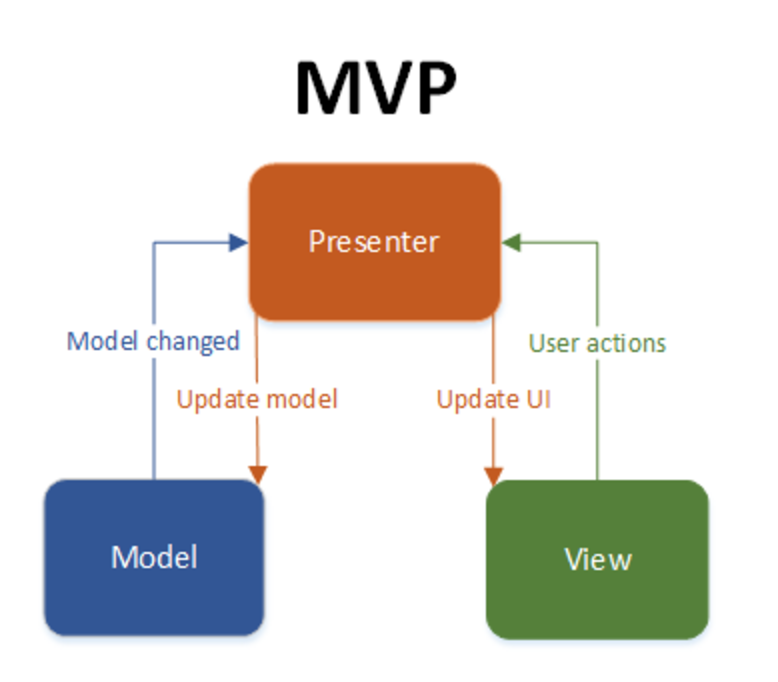
\includegraphics[width=5cm]{imagenes/mvp-basic}
	\end{tabular}
	\\
\end{tabular}

\end{frame}	
%--------------------------------------- 
\begin{frame}[t,fragile]
\frametitle {MVP: Justificación}

\begin{itemize}
	\item Android no recomienda ninguna forma específica de diseñar u organizar la implementación de aplicaciones.
	\vspace{7mm}
	\item No es una buena práctica cargar de lógica a las actividades que se encargan de interactuar	con el usuario.
	\vspace{7mm}
	\item Deberían ser clases por las cuales simplemente la información que interactúa entre el sistema y el usuario fluye.
\end{itemize}
\vspace{3mm}
\begin{center}
	$\Rightarrow$ \textbf{Enseñanza: } tomar un tiempo para elegir la arquitectura antes de comenzar con el desarrollo.

\end{center}

\end{frame}	
%--------------------------------------- 
%\begin{frame}[t,fragile]
%\frametitle {MVP: IMachineApp}
%\begin{figure}[t]
%	\begin{center}
%		\includegraphics[width=0.8\textwidth]%
%		{imagenes/mvp-imachineapp}
%	\end{center}
%\end{figure}
%\end{frame}	 
%--------------------------------------- 
\subsection{Motor de procesamiento de las imágenes}
%---------------------------------------

\watermarkon
\begin{frame}
\frametitle{Agenda}

\tableofcontents[currentsection,currentsubsection]
\end{frame}
\watermarkoff


%---------------------------------------

\begin{frame}[t,fragile]
\frametitle {Motor de procesamiento de las imágenes}

\begin{itemize}
	\item Se denominó \textbf{CIEngine}.
	\vspace{3mm}
	\item Fue pensado como un módulo independiente.
	\vspace{3mm}
	\item Posible adaptación a otros ambientes:
	\begin{itemize}
		\item Programa escritorio.
		\item Servicio alojado en la nube.
		\item Aplicación nativa en otros sistemas operativos utilizados en dispositivos móviles.
	\end{itemize}
	\item Se dividió en 4 etapas:
\end{itemize}
\begin{figure}[t]
	\begin{center}
		\includegraphics[width=0.9\textwidth]%
		{imagenes/ciengine-abstract2}
	\end{center}
\end{figure}
\end{frame}
%---------------------------------------
\begin{frame}[t,fragile]
\frametitle {Extracción de características}
\begin{tabular}{cl}  
	\begin{tabular}{l}
		\parbox{0.5\linewidth}{
			\begin{itemize}
				\item Se utilizó un modelo de \textbf{CNN} denominado MobileNet:
				\vspace{3mm}
				\begin{itemize}
					\item Se encuentra preparado y optimizado para ser utilizado en dispositivos móviles.
					\vspace{2mm}
					\item Puede descargarse una versión pre-entrenada.
					\vspace{2mm}
					\item Puede ser adaptado según la necesidad del proyecto. 
					\vspace{2mm}
					\item El tamaño final de la red utilizada es de 16.9MB.
				\end{itemize}
				%	\item Por cada imagen se obtiene
				%	\item Por cada etiqueta y probabilidad:
				%	\begin{enumerate}
				%		\item Se buscan las 4 etiquetas padres (jerarquía definida por BD WordNet)
				%	\end{enumerate}
			\end{itemize}
		}
	\end{tabular} 
	&
	\begin{tabular}{c}
		
\includegraphics[width=5cm]{imagenes/tensorflow}
	\end{tabular}
	\\
\end{tabular}
\end{frame}
%---------------------------------------
\begin{frame}[t,fragile]
\frametitle {MobileNet}
\begin{itemize}
	\item Fue entrenada con 1001 grupos pertenecientes a la base de datos \textbf{ImageNet}.
	\item A partir de una imagen de entrada, devuelve la probabilidad de que la imagen pertenezca a alguna de las 1001 clases conocidas.
\end{itemize}
\begin{figure}[t]
	\begin{center}
		\includegraphics[width=0.65\textwidth]%
		{imagenes/MobileNet2}
	\end{center}
\end{figure}
\end{frame}
%---------------------------------------
\begin{frame}[t,fragile]
\frametitle {MobileNet}
\begin{itemize}
	\item Dichos grupos están organizados acorde a una jerarquía de etiquetas, provenientes de una base de datos llamada \textbf{WordNet}.
	\item Jerarquía: parten desde una genérica, hacia el detalle en concreto.
\end{itemize} 
\begin{figure}[t]
	\begin{center}
		\includegraphics[width=0.5\textwidth]%
		{imagenes/WordNetExample}
	\end{center}
\end{figure}
\end{frame}
%---------------------------------------
\begin{frame}[t,fragile]
\frametitle {Etapa 1: pre-procesamiento y extracción de características}
\begin{figure}[t]
	\begin{center}
		\includegraphics[width=0.7\textwidth]%
		{imagenes/ciengine-paso1v2}
	\end{center}
\end{figure}
\end{frame}
%---------------------------------------
\begin{frame}[t,fragile]
\frametitle {Pre-procesamiento de las imágenes}
Para todas las imágenes:
\begin{enumerate}
	\item Carga en memoria (bajando su resolución).
	\item Se hace un re-escalado.
	\item Convierte en un arreglo de bytes.
\end{enumerate} 
\begin{figure}[t]
	\begin{center}
		\includegraphics[width=0.7\textwidth]%
		{imagenes/preProcessing}
	\end{center}
\end{figure}
\end{frame}

%---------------------------------------
%\begin{frame}[t,fragile]
%\frametitle {Etapa 1: Pre-procesamiento y extracción de características}
%\begin{figure}[t]
%	\begin{center}
%		\includegraphics[width=0.8\textwidth]%
%		{imagenes/ciengine-paso1}
%	\end{center}
%\end{figure}
%\end{frame}
%---------------------------------------
\begin{frame}[t,fragile]
\frametitle {Resultado 1: etiquetas y probabilidades}
Por cada imagen:
\begin{enumerate}
	\item Se obtiene una lista de hasta 5 etiquetas cuyas probabilidades fueron las más altas.
	\vspace{2mm}
	\item Por cada una de ellas se obtienen hasta 4 etiquetas ``padres'' según \textbf{WordNet}, asignándole la misma probabilidad que la ``hija''.
\end{enumerate}
\begin{figure}[t]
	\begin{center}
		\includegraphics[width=0.5\textwidth]%
		{imagenes/MobileNet2}
		\includegraphics[width=0.4\textwidth]%
		{imagenes/WordNetExample}
	\end{center}
\end{figure}
\end{frame}
%---------------------------------------
\begin{frame}[t,fragile]
\frametitle {Resultado 2: caracterización de las imagenes}	
Por cada imagen:
\begin{itemize}
	\item Se obtiene el vector de \textit{embeddings}.
\end{itemize}
\begin{block}{}
	Los \textit{embeddings} representan como se activó la última capa antes de realizar la clasificación.% y puede ser utilizada como una representación vectorial que la red asimiló para poder caracterizar a la imagen procesada.
\end{block}
\begin{figure}[t]
	\begin{center}
		\includegraphics[width=0.4\textwidth]%
		{imagenes/embeddings}
		\includegraphics[width=0.5\textwidth]%
		{imagenes/deep-learning-model}
	\end{center}
\end{figure}
\end{frame}
%---------------------------------------
\begin{frame}[t,fragile]
\frametitle {Resultado final de la etapa 1}
\vspace{12mm}
\begin{block}{}
	Por cada imagen se obtiene: 
	\vspace{2mm}
	\begin{itemize}
		\item Un conjunto de etiquetas y probabilidades.
		\vspace{1.5mm}
		\item Un vector caracterizador.
	\end{itemize}
\end{block}

\end{frame}
%---------------------------------------
\begin{frame}[t,fragile]
\frametitle {Etapa 2: Medición de similitud}
\begin{itemize}
	\item Se mide el grado de similitud por cada par de imágenes basándose en:
	\vspace{3mm}
	\begin{enumerate}
		\item Las etiquetas y probabilidades de cada una. $\rightarrow$ \textbf{Afinidad gramatical}
		\vspace{3mm}
		\item El vector caracterizador de cada una. $\rightarrow$ \textbf{Afinidad según \textit{embeddings}}
	\end{enumerate}
	\vspace{6mm}
	\item Se registra en una matriz el grado de similitud entre cada par de imágenes \textbf{promediando} las 2 anteriores.
\end{itemize}
\vspace{6mm}
\begin{center}
	$\Rightarrow$ Resultado: \textbf{Matriz de afinidad entre imágenes}
\end{center}
\end{frame}
%--------------------------------------- 
\begin{frame}[t,fragile]
\frametitle {Etapa 3: Ejecución algoritmo de clustering}
\vspace{5mm}
\begin{figure}[t]
	\begin{center}
		\includegraphics[width=1\textwidth]%
		{imagenes/mcl}
	\end{center}
\end{figure}
\vspace{5mm}
\begin{center}
	$\Rightarrow$ Resultado: \textbf{Matriz final de clustering}
\end{center}
\end{frame}
%--------------------------------------- 
\begin{frame}[t,fragile]
\frametitle {Etapa 4: Post-proceso}
Debido al origen de muchos grupos con 1 sola imagen, por cada una de ellas:
\begin{itemize}
	\item Se busca en la matriz de afinidad (previo a la realización del \textit{clustering}) aquella imagen con la que más afinidad comparte, y se la agrega al grupo al cual pertenece la segunda.
	\vspace{6mm}
	\item En caso de no existir ninguna imagen con la cual tenga afinidad, se la junta con aquellas imágenes que cumplen la misma condición.
\end{itemize}

\end{frame}
%---------------------------------------

\subsection{Aplicación Android}
%---------------------------------------

\watermarkon
\begin{frame}
	\frametitle{Agenda}
	
	\tableofcontents[currentsection,currentsubsection]
\end{frame}
\watermarkoff

%\begin{frame}[t,fragile]
%\frametitle {Flujo principal}
%Pantalla inicial:
%\begin{figure}[t]
%	\begin{center}
%		\includegraphics[width=0.3\textwidth]%
%		{imagenes/imachineapp1}
%	\end{center}
%\end{figure}
%\end{frame}
%%---------------------------------------
%\begin{frame}[t,fragile]
%\frametitle {Flujo principal}
%Selección de carpeta/s a procesar:
%\begin{figure}[t]
%	\begin{center}
%		\includegraphics[width=0.3\textwidth]%
%		{imagenes/imachineapp2}
%		\includegraphics[width=0.3\textwidth]%
%		{imagenes/imachineapp3}
%		\includegraphics[width=0.3\textwidth]%
%		{imagenes/imachineapp4}
%	\end{center}
%\end{figure}
%\end{frame}
%%---------------------------------------
%\begin{frame}[t,fragile]
%\frametitle {Flujo principal}
%Procesamiento de las imágenes:
%\begin{figure}[t]
%	\begin{center}
%		\includegraphics[width=0.3\textwidth]%
%		{imagenes/imachineapp5}
%	\end{center}
%\end{figure}
%\end{frame}
%%---------------------------------------
%\begin{frame}[t,fragile]
%\frametitle {Flujo principal}
%Administración de las carpetas resultantes: 
%\begin{figure}[t]
%	\begin{center}
%		\includegraphics[width=0.3\textwidth]%
%		{imagenes/imachineapp6}
%		\includegraphics[width=0.3\textwidth]%
%		{imagenes/imachineapp7}
%		\includegraphics[width=0.3\textwidth]%
%		{imagenes/imachineapp8}
%	\end{center}
%\end{figure}
%\end{frame}
%%---------------------------------------
%\begin{frame}[t,fragile]
%\frametitle {Flujo principal}
%Administración de las imágenes: 
%\begin{figure}[t]
%	\begin{center}
%		\includegraphics[width=0.3\textwidth]%
%		{imagenes/imachineapp9}
%		\includegraphics[width=0.3\textwidth]%
%		{imagenes/imachineapp10}
%		\includegraphics[width=0.3\textwidth]%
%		{imagenes/imachineapp11}
%	\end{center}
%\end{figure}
%\end{frame}
%%---------------------------------------
%\begin{frame}[t,fragile]
%\frametitle {Flujo principal}
%Finalizar la edición: 
%\begin{figure}[t]
%	\begin{center}
%		\includegraphics[width=0.3\textwidth]%
%		{imagenes/imachineapp12}
%	\end{center}
%\end{figure}
%\end{frame}
%%---------------------------------------
%\begin{frame}[t,fragile]
%\frametitle {Flujo principal}
%Administración del resultado: 
%\begin{figure}[t]
%	\begin{center}
%		\includegraphics[width=0.3\textwidth]%
%		{imagenes/imachineapp13}
%		\includegraphics[width=0.3\textwidth]%
%		{imagenes/imachineapp14}
%	\end{center}
%\end{figure}
%\end{frame}
%---------------------------------------
\begin{frame}[t,fragile]
\frametitle {Demo - Ejemplo de uso}
\begin{figure}[t]
	\centering
	\begin{center}
		\includegraphics[width=0.4\textwidth]%
		{imagenes/demotime2}
	\end{center}
\end{figure}
\end{frame}
%---------------------------------------
\begin{frame}[t,fragile]
\frametitle {Otras características}
\begin{tabular}{cl}  
	\begin{tabular}{l}
		\parbox{0.5\linewidth}{
			\begin{itemize}
				\item Manejo de excepciones:
				\begin{itemize}
					\item Si se presiona el botón procesar sin elegir directorio.
					\item Si se elige ver resultados anteriores y no existen.
					\item Se realiza un control de espacio de almacenamiento disponible.
				\end{itemize} 
				\item Multi-idioma: Español e Inglés
			\end{itemize}
		}
	\end{tabular} 
	&
	\begin{tabular}{c}
		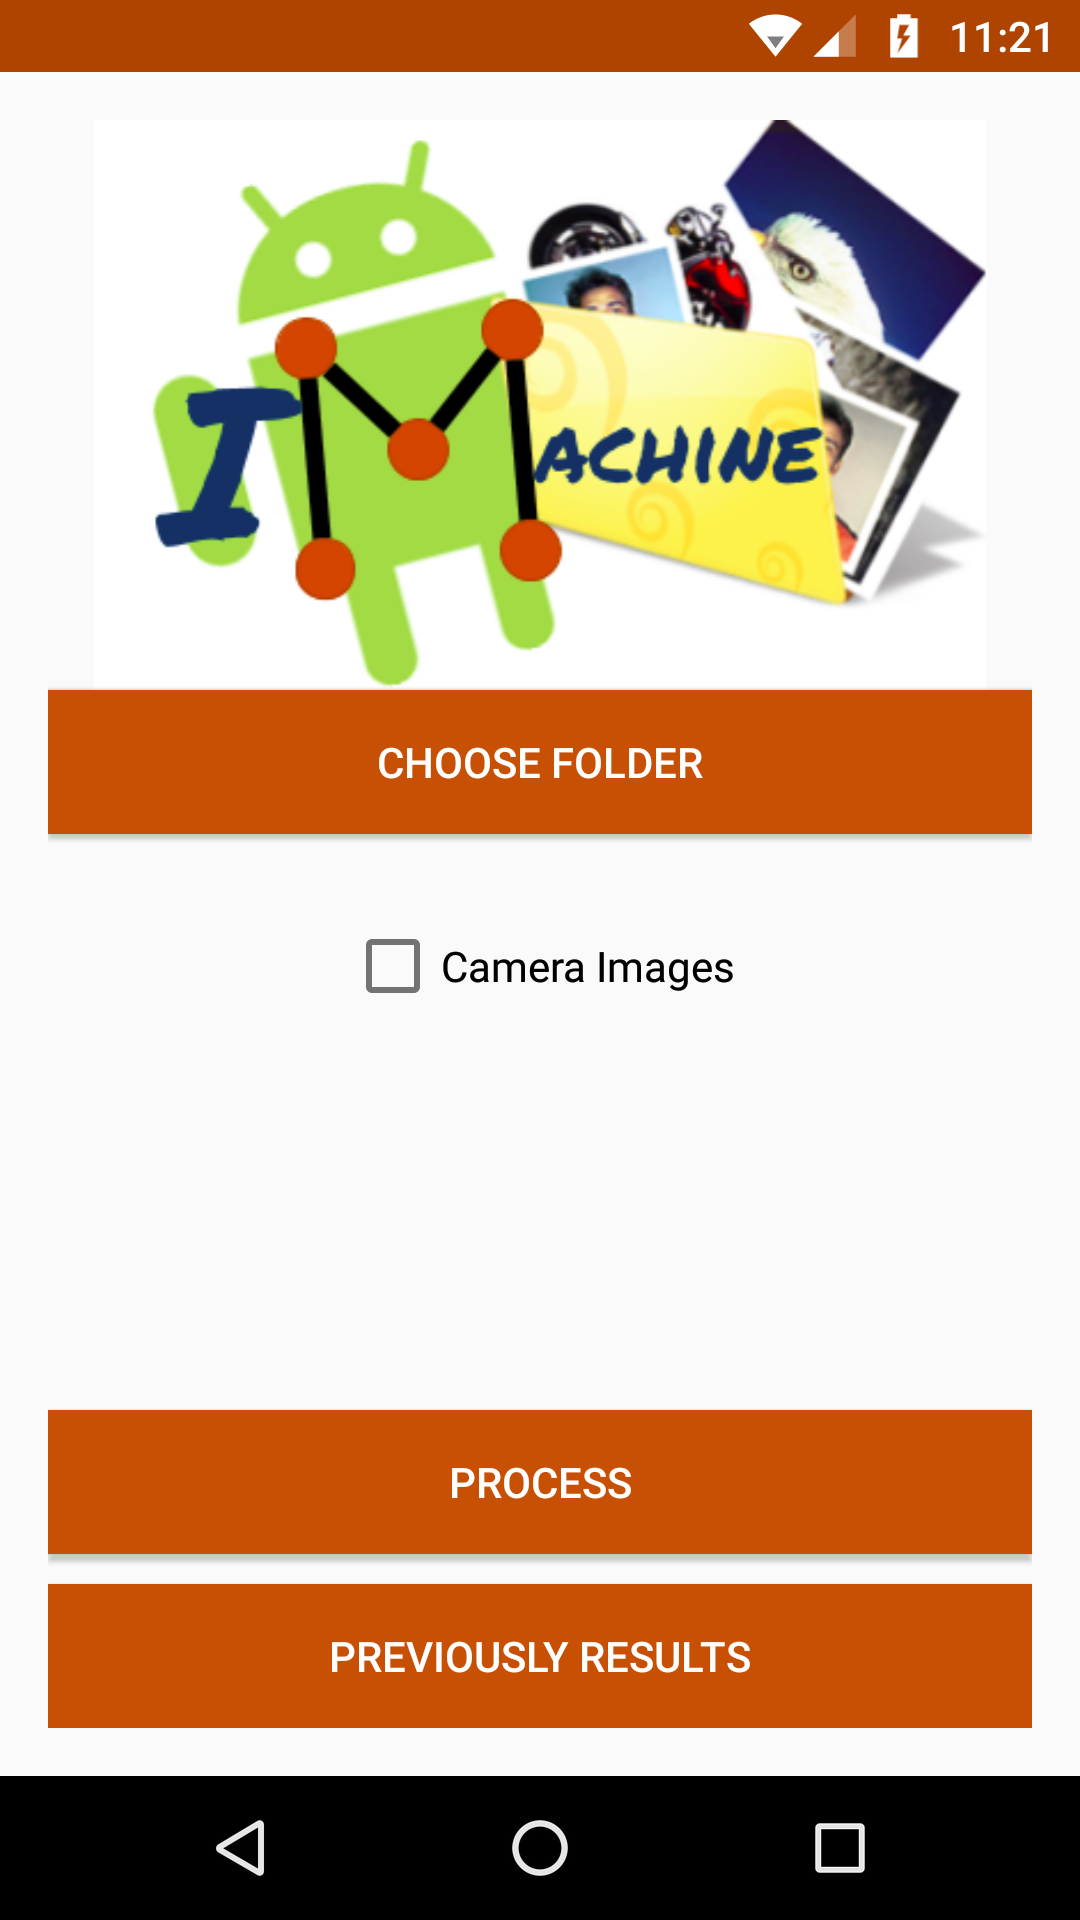
\includegraphics[width=4cm]{imagenes/imachineapp-english}
	\end{tabular}
	\\
\end{tabular}
\end{frame}
%--------------------------------------- 
\section{Evaluación de desempeño}
%---------------------------------------

%--------------------------------------- 
\subsection{Datos usados para la experimentación}
%---------------------------------------

\watermarkon
\begin{frame}
\frametitle{Agenda}

\tableofcontents[currentsection,currentsubsection]
\end{frame}
\watermarkoff

\begin{frame}[t,fragile]
\frametitle {Datos usados para la experimentación}
\begin{itemize}
	\item Imágenes de WhatsApp del ejecutor del proyecto: 1.600 imágenes.
	\item Imágenes del portal de Internet 9GAG: 2.000 imágenes.
	\item Base de datos VOC: 17.000 imágenes
\end{itemize}
\begin{figure}
	\centering
	\begin{center}
		\includegraphics[width=0.6\textwidth]%
		{imagenes/basededatos2}
	\end{center}
\end{figure}
\end{frame}
%---------------------------------------
\subsection{Protocolo de experimentación}
%---------------------------------------

\watermarkon
\begin{frame}
\frametitle{Agenda}

\tableofcontents[currentsection,currentsubsection]
\end{frame}
\watermarkoff

\begin{frame}[t,fragile]
\frametitle {Protocolo de experimentación}
\begin{itemize}
	\item Métricas:
	\begin{itemize}
		\item No se espera tener un desempeño específico en términos de calidad de \textit{clustering}, por lo que no fue necesario realizar una comparación con el estado del arte en dicha tarea.
		\vspace{2mm}
		\item Métricas utilizadas - \color{red} Clasificación \color{black}y \color{blue} Clustering:
		\vspace{2mm}
		\begin{enumerate}
			\item \color{red} Precisión, Recall, F1 Score, Accuracy
			\item \color{blue} Sorensen-Dice, Silhouette 
		\end{enumerate}
	\end{itemize}
	\vspace{3mm}
	\item Desempeño computacional: se midió el tiempo utilizado por cada prueba en diferentes dispositivos móviles:
	\begin{itemize}
		\item Motorola Moto G4 PLUS (Gama media/baja)
		\vspace{2mm}
		\item Xiamoi Redmi Note 4 (Gama media/alta)
		\vspace{2mm}
		\item Samsung Galaxy S9 (Gama alta)
	\end{itemize}
\end{itemize}
\end{frame}
%---------------------------------------
\begin{frame}[t,fragile]
\frametitle {Prueba Nº 1}
Se utilizaron 184 imágenes distribuidas en 6 clases diferentes:
\begin{itemize}
	\item \textbf{Accuracy:} 83.69\%
\end{itemize}
\begin{table}[t]
	\begin{center}
		\label{tab:prueba1}
		\begin{adjustbox}{max width=\textwidth}
			\begin{tabular}{l|c|c|c|c}
				\textbf{Categoría} & \textbf{Cant. Ejemplos} & \textbf{Precision[\%]} & \textbf{Recall[\%]} & \textbf{F1-Score[\%]} \\
				\hline
				Avión & 25 & 95.83 & 95.83 & 95.83\\
				
				Computadora & 35 & 82.85 & 85.29 & 84.06\\
				
				Documento & 50 & 86.53 & 91.83 & 89.11\\
				
				Bebida & 30 & 66.67 & 62.07 & 64.29\\
				
				Fiestas & 33 & 88.89 & 1 & 94.12\\
				
				Estadio & 11 & 70 & 70 & 70\\
				
				Macro-averaging &  & \textbf{81.79} & \textbf{84.17} & \textbf{82.90}\\
				\hline	
			\end{tabular}
		\end{adjustbox}
	\end{center}
\end{table}
\begin{itemize}
	\item \textbf{Silhouette:} 0.25
	\item \textbf{Sorensen-Dice:} 0.83
\end{itemize}
\end{frame}
%---------------------------------------
\begin{frame}[t,fragile]
\frametitle {Prueba Nº 1}
\vspace{10mm}
\begin{table}[t]
	\begin{center}
		\label{tab:tiempo1}
		\begin{adjustbox}{max width=\textwidth}
			\begin{tabular}{l|c}
				\hline
				\hline
				\textbf{Dispositivo} & \textbf{Tiempo de proceso (segundos)}\\
				\hline
				Moto G4 Plus & 142.75\\
				
				Xiaomi Redmi 4 & 88.31\\
				
				Samsung Galaxy S9 & 35.86\\
				\hline
			\end{tabular}
		\end{adjustbox}
	\end{center}
\end{table}
\vspace{5mm}
\begin{center}
	$\Rightarrow$ Cuanto mayor es la gama del dispositivo, menor es el tiempo de proceso
\end{center}
\end{frame}
%---------------------------------------
\begin{frame}[t,fragile]
\frametitle {Prueba Nº 2}
\begin{itemize}
	\item Se utilizaron 298 imágenes divididas en 5 grupos:
	\begin{itemize}
		\item \textbf{\color{red}Accuracy:} 55.7\%
		\item \textbf{\color{red}Precision:} 56.5\%
		\item \textbf{\color{red}Recall:} 62.5\%
		\item \textbf{\color{red}F1-Score:} 59.2\%
		\item \textbf{\color{blue}Silhouette:} 0.01\%
		\item \textbf{\color{blue}Sorensen-Dice:} 0.58\%
	\end{itemize}
\end{itemize}
\begin{table}[h!]
	\begin{center}
		\label{tab:tiempo2}
		\begin{adjustbox}{max width=\textwidth}
			\begin{tabular}{l|c}
				\hline
				\hline
				\textbf{Dispositivo} & \textbf{Tiempo de proceso (segundos)}\\
				\hline
				Moto G4 Plus & 215.24\\
				
				Xiaomi Redmi 4 & 138.20\\
				
				Samsung Galaxy S9 & 62.25\\
				\hline
			\end{tabular}
		\end{adjustbox}
	\end{center}
\end{table}
\end{frame}
%---------------------------------------
\begin{frame}[t,fragile]
\frametitle {Prueba Nº 3}
\begin{itemize}
	\item \small{\textbf{\color{red}Accuracy:} 63\%}
	\item \small{\textbf{\color{blue}Silhouette:} 0.16\%}
	\item \small{\textbf{\color{blue}Sorensen-Dice:} 0.63\%}
\end{itemize}
\begin{figure}[t]
	\centering
	\begin{center}
		\includegraphics[width=0.75\textwidth]%
		{imagenes/prueba3-1}
	\end{center}
\end{figure}
\begin{figure}[t]
	\centering
	\begin{center}
		\includegraphics[width=0.5\textwidth]%
		{imagenes/prueba3-2}
	\end{center}
\end{figure}
\end{frame}

%---------------------------------------
\begin{frame}[t,fragile]
\frametitle {Validación de la aplicación}
\begin{itemize}
	\item \small{Se implementó un esquema automatizado de testeo realizando \textit{unit testing}.}
	\begin{figure}[t]
		\centering
		\begin{center}
			\includegraphics[width=0.25\textwidth]%
			{imagenes/testing2}
		\end{center}
	\end{figure}
	\item \small{Se realizó un protocolo de validación de todos los módulos que componen la aplicación, con el objetivo de validar que se comporta y actúa según lo esperado.}
	\pause
	
	\begin{figure}[t]
		\begin{center}
			\includegraphics[width=0.75\textwidth]%
			{imagenes/prot-validacion-ej2}
		\end{center}
	\end{figure}
\end{itemize}



\end{frame}
%#######################################################

\section{Conclusiones y discusión}


\watermarkon
\begin{frame}
	\frametitle{Agenda}
	
	\tableofcontents[currentsection,currentsubsection]
\end{frame}
\watermarkoff


%---------------------------------------
\begin{frame}[t,fragile]
\frametitle {Conclusiones}

	\begin{itemize}
		\item \small{Producto de software sobre la plataforma Android que, sin la necesidad de una conexión a Internet y a partir de imágenes almacenadas en el dispositivo, sugiera una estructura de directorios para organizar el conjunto}
		\vspace{3mm}
		\item Provee funcionalidades que le permiten al usuario la interacción con el resultado anterior, adecuándolo a sus preferencias.
		\vspace{3mm}
		\item Aprendizaje de nuevas tecnologías: 
		
		\begin{itemize}
			\item Herramientas para construir la aplicación (e.g. Java, SDK Android)
			
			\item Patrón de diseño de software: MVP
			
			\item Algoritmos de \textit{computer vision} y \textit{clustering} implementados (e.g APIs de TensorFlow, MobileNet, ImageNet, MCL).
		\end{itemize}
		
	\end{itemize}
\end{frame}

%---------------------------------------
%\begin{frame}[t,fragile]
%\frametitle {Conclusiones}
%
%\begin{figure}
%	\centering
%	\begin{tikzpicture}
%	\pie[text=legend, radius=2.5]{35/Programación, 20/Software, 30/Aplicación, 15/Matemáticas}
%	\end{tikzpicture}
%	
%	\caption{Gráfico de torta con las contribuciones de cada área curricular hacia el proyecto desarrollado (calculadas en forma subjetiva).}
%	\label{fig:pie-plot-asignaturas}
%\end{figure}
%
%\end{frame}
%---------------------------------------
\begin{frame}[t,fragile]
\frametitle {Trabajos futuros}
Se consideran las siguientes cuestiones a mejorar en un futuro:

\begin{itemize}
	\item Incorporar nuevas características para describir mejor las imágenes.
	\vspace{4mm}
	\item Estudiar metodologías para aumentar el número de imágenes a procesar a la vez.
	\vspace{4mm}
	\item Reducir el consumo de almacenamiento y memoria.
	\vspace{4mm}
	\item Dar un nombre representativo a cada carpeta.
	\vspace{4mm}
%	\item Aumentar la cantidad de pruebas unitarias.
	
%	\item Implementar un proceso de integración continua.
	
	\item Extender el uso del motor de procesamiento hacia otras plataformas (e.g Desktop, iOS, Cloud)
\end{itemize}
\end{frame}

%---------------------------------------
\begin{frame}[t,fragile]
\frametitle {Preguntas}
\begin{block}{}
   	\usebeamerfont{title} \centering ¡Muchas gracias por su atención!\\
\end{block}

\begin{figure}[t]
\centering
\begin{center}
	\includegraphics[width=0.8\textwidth]%
	{imagenes/preguntas}
\end{center}
\end{figure}
		
\end{frame}
\end{document}

